\documentclass[9pt,twoside,lineno]{pnas-new}
% Use the lineno option to display guide line numbers if required.
\usepackage{mathptmx}	
\usepackage{nicefrac}
\usepackage{amsmath}
\usepackage{amsfonts}
\usepackage{amsthm}
\usepackage{amssymb}
\usepackage{bbm}
\usepackage[hidelinks]{hyperref}
\usepackage[linesnumbered,ruled]{algorithm2e}
\usepackage{color}
\usepackage{graphicx}
%\usepackage[export]{adjustbox}
\usepackage{float}
\usepackage{caption}
\usepackage{enumerate}
\captionsetup{font=footnotesize}
\renewcommand{\thefigure}{S\arabic{figure}}
\renewcommand{\thetable}{S\arabic{table}}

\makeatletter
\newcommand{\algorithmfootnote}[2][\footnotesize]{%
	\let\old@algocf@finish\@algocf@finish% Store algorithm finish macro
	\def\@algocf@finish{\old@algocf@finish% Update finish macro to insert "footnote"
		\leavevmode\rlap{\begin{minipage}{\linewidth}
				#1#2
		\end{minipage}}%
	}%
}
\makeatother

\usepackage{easy-todo}

\DeclareMathOperator{\di}{d\!}
\newcommand*\Eval[3]{\left.#1\right\rvert_{#2}^{#3}}

%\usepackage[backend=biber,style=apa]{biblatex}
%\DeclareLanguageMapping{british}{british-apa}
%\usepackage{epigraph}
%\usepackage{dsfont}
\usepackage{setspace}
\usepackage{cleveref}
\usepackage{natbib}
\usepackage{etoolbox}
\usepackage[margin=1in]{geometry}
%\setlength{\epigraphwidth}{5.5in}
\usepackage{accents}
\usepackage{lscape}
\usepackage[normalem]{ulem}
\useunder{\uline}{\ul}{}

\newcommand{\ubar}[1]{\underaccent{\bar}{#1}}
\newcommand\addtag{\refstepcounter{equation}\tag{\theequation}}

\newtheorem{prop}{Proposition}
\newtheorem{lemm}{Lemma}
\newtheorem{thm}{Theorem}
\newtheorem{conj}{Conjecture}
\newtheorem{assn}{Assumption}
\newtheorem{defn}{Definition}
\newtheorem{coro}{Corollary}

\templatetype{pnassupportinginfo}

\title{Orbital-use fees could more than quadruple the value of the space industrye}
\author{Akhil Rao, Matthew Burgess, Daniel Kaffine}
\correspondingauthor{Akhil Rao.\\E-mail: akhilr@middlebury.edu}

\begin{document}

%% Comment/remove this line before generating final copy for submission; this will also remove the warning re "Consecutive odd pages found".
\instructionspage  

\maketitle

%% Adds the main heading for the SI text. Comment out this line if you do not have any supporting information text.
\SItext


%\subsection*{Subhead}
%Type or paste text here. This should be additional explanatory text such as an extended technical description of results, full details of mathematical models, etc.   

\section*{Extended description of methods and discussion of results}

% What are we doing?
We generate the path of an optimal orbital-use fee (OUF) in three steps. First, we calibrate functions describing the physics and economics of orbit use to match observed data on satellite and debris stock levels and aggregate satellite industry costs and returns prior to 2015. Then, using the calibrated values, we generate open access and optimal launch paths from 2006 to 2040. Finally, by comparing the open access path of collision risk to the optimal path of collision risk, we calculate the path of the optimal OUF which induces open access satellite owners to internalize the externality they impose on other orbit users. \\

% What is this saying?
It is important to emphasize that our goal in this article is not to precisely estimate the value of an OUF. Rather, our goal is to provide order-of-magnitude estimates of the optimal OUF and the NPV gains from implementing it, and to show the qualitative features of both the OUF path and NPV gains. As we discuss below, our conclusion that a globally-harmonized OUF is necessary to improve the value of the satellite industry is robust to the limitations in our estimation methodology.\\ 

% More detailed ``what are we doing''?
We measure the value of the satellite industry as the net present value (NPV) of cash flows generated by the satellite fleet. NPV accounts for the time value of money --- the fact that cash flows received sooner are preferable to cash flows received later --- by discounting future cash flows according to the interest that could have been earned on those cash flows had they been received in the present and immediately reinvested in capital markets. In this article, we use the infinite-horizon NPV of the satellite fleet. To calculate this value, we assume that satellite costs and revenues evolve according to the projection in \citet{MSreport} until 2050, after which they stabilize at 2050 levels and are constant for the infinite future.\footnote{The projection in \citet{MSreport} only goes till 2040 --- we extend it to 2050 by calculating the compound annual growth rate of the costs and revenues, and assuming that they continue to grow at those rates from 2040 until 2050.} The resulting NPVs reflect the sum of short- and long-run costs and returns from the satellite fleet. To express these in terms of equivalent constant cash flows received each year, we convert the NPV into an annuitized present value in the main text.\footnote{The annuitized present value (PV) of an NPV level is the constant number of dollars received each year such that the discounted sum of annuitized PVs is equal to the target NPV level. Formally, defining the NPV of a stream of uneven cashflows $x_t$ as $NPV = \sum_{t=1}^{\infty} \beta^{t-1} x_t = \sum_{t=1}^{\infty} \beta^{t-1} A = A(1 - \beta)^{-1}$ for some constants $A>0$ and $\beta \in (0,1)$, the annuitized PV is $A = NPV(1-\beta)$. These conversions facilitate comparisons between uneven streams of cash flows, as they can be expressed in a common unit at a single point in time (NPV terms) or in a common unit at every point in time (annuitized PV terms).}  For example, given a discount rate of 5\%, a net present value of \$1 trillion in 2020 is equivalent to an annuitized present value of \$47 billion received in perpetuity in each year from 2020 onwards.\footnote{We discuss the interpretation of the discount rate as the opportunity cost of funds invested below.} \\

%Paragraph 2: high-level overview of how we're doing it \\
We obtain physical functions relating launches, satellites, and debris stocks to collisions, new fragments, and satellite and debris growth from the engineering literature, and economic functions relating the decision to launch to collision risk, costs, and returns from the economics literature. To calibrate the physical functions, we estimate the unknown parameters from satellite stocks, debris stocks, and launches observed over 1957--2017. We constrain the parameters to comply with theoretical restrictions imposed by the engineering model. To calibrate the economic functions, we estimate the unknown parameters from satellite stocks, debris stocks, launches, aggregate satellite industry costs, and aggregate satellite industry returns over 2005--2015. To allow the estimation process to adjust for unobserved launch market frictions, we do not constrain these parameter estimates. 

\subsection{Data}

\subsubsection{Satellite and debris counts, 1957--2015}

We use data on satellites in orbit from the Union of Concerned Scientists' (UCS) lists of active satellites to construct the satellite stock and launch rate series \citep{UCSdata}. The UCS data provide details on payloads in low-Earth orbit (LEO) and their projected lifetimes. The data are described in Extended Data Table 1. \\

%We use data on satellites in orbit from the Space-Track dataset hosted by the Combined Space Operations Center (CSpOC) \citep{spacetrackData} to construct the satellite stock and launch rate series. The Space-Track dataset provides details on active payloads in low-Earth orbit (LEO) and their decay dates. The data are described in Extended Data Table 1. \\
%Table \ref{physstock_sumstat}.\\

We construct the numbers of active satellites in each year by calculating the number of objects launched a particular year, adding the number of satellites previously calculated in orbit, and then subtracting the number of satellites listed as having decayed in that year.\footnote{This procedure is likely to produce an upward-biased estimate of the returns-generating satellite stock in any given year, since satellites which are no longer operational will not be removed from the estimated stock until they have deorbited. Thus, the satellite stock in this procedure includes some objects which are, economically speaking, ``socially-useless debris''. We use this procedure despite the attribution issue for two reasons. First, we do not have data on when specific satellites were declared nonoperational by their owners. Such a determination can be particularly tricky when a mission has ended, but the satellite still has fuel and could be repurposed for another mission. Second, to the extent that our estimates of the satellite stock are biased upward (toward positive infinity), our physical and economic parameters estimates will be biased downwards. The downward bias in economic parameters will deflate both the open access and socially optimal launch rates, while the downward bias in physical parameters will inflate both the open access and socially optimal launch rates, with the net effect being difficult to determine. However, the downward bias in our estimated collision risk coefficients and the upward bias in our estimated satellite stock will bias our estimated OUF downward, so that it is a lower bound.} \\

%We use data on satellites in orbit from the Space-Track dataset hosted by the Combined Space Operations Center (CSpOC) \citep{spacetrackData} to construct the satellite stock and launch rate series. The Space-Track dataset provides details on active payloads in LEO and their decay dates. We construct the numbers of active satellites in each year by calculating the number of objects launched a particular year, adding the number of satellites previously calculated in orbit, and then subtracting the number of satellites estimated to be nonoperational. We attribute operational status to satellites based on the number of years since the satellite's launch: if a satellite was launched at year $t$ with a lifespan of $\hat{t}$ years, then the satellite will be declared nonoperational in year $t + \hat{t}$. 

Letting $\ell_t$ be the number of collisions observed in year $t$ and $Z_t$ be the number of payloads listed as decayed in $t$, we construct the launch rate in $t$, $X_t$, from the law of motion for the satellite stock series as
\begin{align}
S_{t+1} &= S_t - Z_t - \ell_t + X_t \nonumber \\
\implies X_t &= S_{t+1} - S_t + Z_t + \ell_t,
\label{launchRateAccounting}
\end{align}

where $S_t$ is the number of active payloads in $t$ and $Z_t$ is the number of payloads listed as decayed in $t$. \\

The debris and collision risk series' we use were provided by the European Space Agency. We use debris data from the DISCOS database \citep{FRAGdata} and collision probability data used in \citep{ECOBdata} (the variable $p_c$ in that paper). We use only objects with a semi-major axis of 2000km or less in all our data series. We prefer to use the DISCOS fragment data rather than the Space-Track fragment data \citep{spacetrackData} as DISCOS considers fragments from the time they were created or detected, whereas the Space-Track data tracks fragments from the time their parent body was launched. The DISCOS attribution method is closer to how economic agents in our model receive information and make decisions. Given the difficulties in determining operational status, the collision probability estimates account for the probability of collisions with all intact bodies. This produces an upward-biased estimate of the probability of collisions with only operational satellites. This upward bias likely deflates the number of open access and optimal launches we project. However, since the open access and optimal launch rates are chosen to equate collision risk with measures of economic returns (described in equations \ref{OAeqm_ch3} and \ref{plannersFOC}), the resulting estimated OUF paths will not be biased upward by the same degree as the collision probability estimates.

\subsubsection{Aggregate satellite industry returns and costs, 2006--2040}

We use data on satellite industry revenues from \citet{wienzierl2018}, and UCS data on satellites in LEO (semi-major axis less than 2000km) \citep{UCSdata}. The economic data provide a breakdown of revenues across satellite manufacture, launch, insurance, and products and services. The satellite industry revenues data cover 2006-2015, while the active satellites data cover 1958-2017. To generate launch rate and OUF projections out to 2040, we use revenue and cost projections from \citet{MSreport}. These projections are shown in Figure 1a of the main text. The historical and projected data are described in Extended Data table 1. \\

We calculate the per-period returns on owning a satellite ($\pi_t$) as the revenues generated from commercial space products and services, and the per-period costs of launching a satellite ($F_t$) as the sum of revenues from commercial infrastructure and support industries, ground stations and equipment, commercial satellite manufacturing, and commercial satellite launching. The ratio $\pi_t/F_t$ then gives a time series of the rate of return on a single satellite, as the number of satellites cancels out of the numerator and denominator.\footnote{This is true whether the satellites were launched individually on separate rockets or in groups on the same rockets.} Since the numbers provided in \citet{wienzierl2018} are for the satellite industry as a whole, the ratio still needs to be adjusted to represent satellites in LEO. We do not explicitly conduct this adjustment, but let the adjustment be calculated during the estimation of equation \ref{OAeqm_ch3_2}.\footnote{Another way to perform this adjustment is by calculating the yearly share of satellites in LEO and multiplying the ratio $\pi_t/F_t$ by the share in LEO. This approach is difficult to generalize to future years since it requires projections of satellites in other orbits. It is also not clear that the returns of satellites in LEO are truly proportional to the LEO share of the total number of active satellites in all orbits; it seems more likely that LEO satellites earn less revenue per satellite than geostationary satellites.} \\ %We adjust for this by calculating the yearly share of satellites in LEO and multiplying the ratio by this share. \\ , and runs the risk of ``data-snooping'': since we are trying to predict the launch rate using only economic parameters (returns, costs, interest rates), incorporating the share of satellites in LEO adds physical information to the economic estimation.

Note that the data we use for $\pi_t$ and $F_t$ are industry-level aggregates, rather than satellite-level figures. To convert the data from industry-level figures to per-satellite figures, we must apply a scaling factor which ``disaggregates'' the data. This unknown factor is common to both cost and revenue aggregates, and so cancels out of $\pi_t/F_t$ such that the ratio correctly represents the rate of return per satellite. Since we use $\pi_t/F_t$ to compute the open access and optimal policy and value functions, the unknown scaling factor does not affect our solutions (launch rates). However, it does affect our calculated time paths of NPV under BAU and optimal management as well as the OUF, since those values do not involve ratios which would cancel out the unknown scaling factor. Since the unknown scaling factor is on the order of the reciprocal of the number of satellites in orbit (or projected to be in orbit) in each period, we proxy for it in our projected time paths by dividing by the BAU satellite stock path. This choice of proxy does not affect our qualitative results or the order of magnitude of the OUF or NPV under BAU and optimal management --- using alternate proxies such as the optimal management path of satellites or the observed number of satellites in 2015 produces similar results, although our proxy results in more conservative projections than those alternative choices. % However, to the extent that our BAU time path overstates the number of satellites launched, it makes our projections conservative. We discuss some reasons to believe that our model may overstate the BAU launch rate in section \ref{disc_unmodeledeconphys}.

\subsection{Models}

\subsubsection{Orbital mechanics with limited lifespans, missile tests, and certainty}

Our physical model uses physical accounting relationships in the aggregate stocks of satellites and debris for the laws of motion, and draws on \citep{letiziaetal2017} for the functional forms of the new fragment creation and collision probability functions $G(S,D)$ and $L(S,D)$. The time scale is set as one calendar year to match our data. $S_t$ denotes the number of active satellites in an orbital shell in period $t$, $D_t$ the number of debris objects in the shell in $t$, $X_t$ the number of satellites launched in $t$, $L(S_t,D_t)$ the probability that an active satellite in the shell will be destroyed in a collision in $t$, $\mu$ is the fraction of satellites which do not deorbit in $t$, and $m$ is the average amount of debris generated by launching satellites (such as rocket bodies). $\delta$ is the average proportion of debris objects which deorbit in $t$, and $G(S_t,D_t)$ is the number of new debris fragments generated due to all collisions between satellites and debris.\footnote{For most of our sample, the number of observed collisions is zero. We use the probability of collisions in our models rather than the observed number for two reasons. First, it proxies for unobserved collisions, including non-catastrophic ones. Second, a model with stochastic collisions complicates the process of solving for the optimal time path by adding another state variable to the dynamic programming algorithm. As the number of objects in a single period increases, the fraction of satellites destroyed in collisions in that period converges to the probability of destruction, so this assumption provides a ``mean field''-type approximation.} $A_t$ is the number of anti-satellite missile tests conducted in $t$, and $\gamma$ is the average number of fragments created by one test. We assume that satellites which deorbit do so without creating any additional debris. \\

The number of active satellites in orbit is modeled as the number of launches in the previous period plus the number of satellites which survived the previous period (also shown in equation \ref{launchRateAccounting}). The amount of debris in orbit is the amount from the previous period which did not decay, plus the number of new fragments created in collisions, plus the amount of debris in the shell created by new launches.\footnote{Empirically, we only consider the population of trackable fragments, i.e. those with size greater than 5-10 cm in LEO.} Formally,
\begin{align}
\label{satelliteLoM}
S_{t+1} &= S_t(1 - L(S_t,D_t))\mu + X_t \\
\label{debrisLoM}
D_{t+1} &= D_t(1-\delta) + G(S_t,D_t) + \gamma A_t + mX_t.
\end{align}

For simplicity, we assume all non-operational satellites are immediately deorbited, making our OUF estimates conservative. \cite{letiziaetal2017} use an analogy to kinetic gas theory to parameterize the probability of a collision as a negative exponential function, with the density of colliding objects one of the arguments of the exponential function. We therefore parameterize $L(S_t,D_t)$ as
\begin{equation}
\label{collFunction}
L(S_t,D_t) = 1 - \exp(-\alpha_{SS}S_t - \alpha_{SD}D_t),
\end{equation}

where $\alpha_{SS}$ and $\alpha_{SD}$ include the difference in velocities between the objects colliding, the total cross-sectional area of the collision, and scaling parameters which relate the number of objects to their density in the volume. We use these probability functional forms to parameterize $G(S_t,D_t)$ as

\begin{equation}
\label{growthFunction}
G(S_t,D_t) = \beta_{SS} (1 - \exp(-\alpha_{SS}S_t))S_t + \beta_{SD} (1 - \exp(-\alpha_{SD}D_t))S_t,
\end{equation}

where the $\beta_{jk}$ parameters are interpreted as ``effective'' numbers of fragments from collisions between objects of type $j$ and $k$.\footnote{``Effective'' numbers of fragments measure the number of new fragments weighted by the time they spend inside the volume of interest. This approach is used in the debris modeling literature, for example \cite{bradleywein2009}.} We refer to the $\alpha_{jk}$ and $\beta_{jk}$ as ``structural physics parameters'', as they represent physical entities which are exogenous to our model.\\ 

We ignore the possibility of collisions between debris objects for two reasons. First, the data we have do not allow us to identify the effective number of fragments from such collisions, or the probability of such collisions, using our calibration approach. Second, our focus here is not on the probability of Kessler Syndrome, but on launch patterns and their response to the extant stock of orbiting satellites and debris. Our estimates of the optimal OUF path and the benefits of implementing it are likely understated due to this omission. Incorporating the possibility of Kessler Syndrome is an important piece of optimal orbit use analysis and policy design, and will likely require higher-fidelity physical modeling than the ``aggregate calibration'' approach we take here. This is an important area for future research.\\

Equations \ref{debrisLoM}, \ref{collFunction}, and \ref{growthFunction} can be viewed as reduced-form statistical models which recreate the results of higher-fidelity physics models of debris growth and the collision probability. While higher-fidelity physics models may use similar functional forms, the key difference between our approach and the approach in such models is how we calibrate the models: rather than derive the appropriate parameter values from physical first principles given the data, we estimate the values of those parameters which maximize the fit between the data and model-predicted collision probabilities, satellite evolution, and debris stocks. Though our approach is computationally convenient, it likely sacrifices some predictive power.

\subsubsection{Open access orbit use with time-varying aggregate returns and costs}

The economic model of open access here is based on the model of open access in \cite{rao2019diss} to determine the satellite launch rate under open access, $X_t$, as a function of the collision probability, $L(S_{t+1},D_{t+1})$, and the excess return on a satellite, $r_{s} - r$.\footnote{While we consider LEO as a whole, this approach could be generalized to individual spherical shells within LEO. Such generalization could incorporate the substantial heterogeneity in orbital-use values. For example, some orbits are more valuable because they offer ideal conditions for Earth observation, and will likely need a different fee schedule than orbits which do not offer such conditions.} In the simplest case, where all of the economic parameters are constant over time, the open access launch rate equates the collision probability with the excess return:
\begin{equation}
\label{OAeqm_ch3}
L(S_{t+1},D_{t+1}) = \underbrace{r_s - r}_{\text{\shortstack{excess return\\on a satellite}}},
\end{equation}

where $r_s$ is the per-period rate of return on a single satellite ($\pi/F$, where $\pi$ is the per-period return generated by a satellite and $F$ is the cost of launching a satellite, inclusive of non-launch expenditures such as satellite manufacturing and ground stations) and $r$ is the risk-free interest rate.\footnote{More precisely, $r$ is the opportunity cost of funds invested in launching a satellite, and may diverge from the risk-free rate if the satellite launcher's most-preferred alternate investment is not a risk-free security. This rate is sometimes referred to as the internal rate of return.} \\

Equation \ref{OAeqm_ch3} can therefore also be used to calculate the implied internal rate of return (IRR) for satellite investments from observed data on collision risk and satellite returns. $r$ is not observed in our data. When costs and returns are time-varying, equation \ref{OAeqm_ch3} becomes
\begin{align}
\label{OAeqm_ch3_2}
L(S_{t+1},D_{t+1}) &= 1+ r_{s,t+1} - (1+r) \frac{F_t}{F_{t+1}} \\
\implies L(S_{t+1},D_{t+1}) &= \underbrace{\left( r_{s,t+1} - r \frac{F_t}{F_{t+1}} \right)}_{\text{\shortstack{excess return\\on a satellite}}} + \underbrace{\left(1 - \frac{F_t}{F_{t+1}} \right)}_{\text{\shortstack{capital gains\\from open access\\and satellite launch\\cost variation}}} \nonumber
\end{align}

where $r_{s,t+1} = \pi_{t+1}/F_{t+1}$. With time-varying economic parameters, two sources of returns drive the collision risk. One is the excess return realized in $t+1$ from launching a satellite in $t$. The other is the capital gain (or loss) due to open access and the change in satellite costs. Since open access drives the value of a satellite down to the total cost of launching and operating it, $F_t$ becomes the cost of receiving $F_{t+1}$ in present value the following period, and the returns are given as percentages of $F_{t+1}$. Since the discount rate is unobserved, we fix it to be constant over time to facilitate estimation.\footnote{This equation was derived in the Appendix of \cite{rao2019diss}. In that setting the discount rate was not constant over time.} While we abstract from the fact that satellite lifetimes are finite, this extension was considered in \cite{rao2019diss} and shorter planned operational lifetimes were shown to reduce the expected collision risk. We discuss this issue further when describing our calibration methodology in section \ref{economicCalibrationSection}, including why it is unlikely to affect our estimates of the optimal OUF and the benefits of implementing it.

\subsubsection{Optimal orbit use with time-varying aggregate returns and costs}

Determining the launch plan to ensure optimal orbit use is more complicated. Economists commonly refer to this type of problem as ``the (fleet) planner's problem'', imagining a planner tasked with maximizing fleet-wide NPV. The fleet planner launches satellites to maximize the value of the entire fleet into the (discounted) infinite future, subject to the laws of motion of satellite and debris stocks. Formally, letting $\beta = (1+r)^{-1}$ be the discount factor, the planner solves

\begin{align}
\label{plannersProblem}
W(S,D) &= \max_{X \geq 0} \{ \pi S - F X + \beta W(S',D') \} \\
& S' = S(1 - L(S,D))\mu + X \nonumber \\
& D' = D(1-\delta) + G(S,D) + \gamma A + m X \nonumber .
\end{align}
We drop time subscripts and use primes on a variable's right to indicate future values, in keeping with the convention for infinite-horizon dynamic programming problems. The economic parameters $\pi$ and $F$ are allowed to be time-varying in our solution approach, though all other physical and economic parameters are constant over time. \\

Solving the planner's problem by taking the first-order condition and applying the envelope condition to recover the unknown functional derivatives, we obtain an expression for the collision risk in period $t+1$ which characterizes the optimal launch rate in period $t$:

Combining equation \ref{W_Dformula} with equation \ref{BS_D4} iterated one period forwards, we obtain
\begin{equation}
\label{plannersFOC}
L(S_{t+1},D_{t+1}) = 1 + r_{s,t+1} - (1+r)\frac{F_t}{F_{t+1}} - \xi(S_{t+1},D_{t+1}),
\end{equation}
where
\begin{align}
&\xi(S_{t+1},D_{t+1})  = S_{t+1}L_S(S_{t+1},D_{t+1})F + \frac{\pi - rF - L(S_t,D_t)F - S_t L_S(S_t,D_t) F}{\beta (1- \delta + G_D(S_{t+1},D_{t+1}) + mL_D(S_{t+1},D_{t+1})S_{t+1} )} \nonumber \\ 
& ~~~~~ -\frac{\beta G_S(S_{t+1},D_{t+1}) + m(1 - L(S_{t+1},D_{t+1}) - S_{t+1}L_S(S_{t+1},D_{t+1}))}{\beta (1- \delta + G_D(S_{t+1},D_{t+1}) + mL_D(S_{t+1},D_{t+1})S_{t+1} )}L_D(S_{t+1},D_{t+1})S_{t+1}F
\label{MEC_formula}
\end{align}

is defined as the marginal external cost of another satellite. This equation is derived in the Supplementary Equations.

\subsection{Calibration and simulation}
\subsubsection{Physical parameters: deorbit, decay, collisions, and fragments}

We calibrate the rate at which satellites deorbit, $\mu$, by estimating the following analog to equation \ref{launchRateAccounting} by ordinary least squares (OLS):

\begin{equation}
\label{deorbitRateEstimate}
S_{t+1} = S_t(1-L(S_t,D_t))\hat{\mu} + X_t.
\end{equation}

We use hats over variables to indicate a parameter being estimated, e.g. $\mu$ is the true (unknown) value while $\hat{\mu}$ is the estimate of $\mu$. \\

Equation \ref{deorbitRateEstimate} yields an estimated average lifespan of about 30 years, i.e. $\hat{\mu} = 0.967$. This is consistent with an average mission length of 5 years, followed by compliance with the 25-year deorbit guideline issued by the IADC \citep{IADCdmg}. 
%While only four in five LEO operators who launched between 2003 and 2014 are estimated to comply with the guideline, 
Using this rate in our forward simulations is conservative in the sense that the estimated OUF becomes a lower bound relative to a model with imperfect compliance, given that \citet{bradleywein2009} show full compliance to be optimal. \\

We calibrate equations \ref{collFunction} and \ref{debrisLoM} by estimating the following equations:
\begin{align}
\label{riskEstimation}
L(S_t,D_t) &= 1 - \exp(-\hat{\alpha}_{SS} S_t-\hat{\alpha}_{SD} D_t) + \epsilon_{L t}  \\
\label{debLoMEstimation}
D_{t+1} &= \hat{(1-\delta)} D_t + \hat{\beta}_{SS} (1-\exp(-\hat{\alpha}_{SS}S_t))S_t + \hat{\beta}_{SD} (1-\exp(-\hat{\alpha}_{SD}D_t))S_t + \\
&~~~~~  \hat{\gamma} A_t + \hat{m} X_t + \epsilon_{D t},
\end{align}

where $\epsilon_{xt}$ are mean-zero error terms to minimize and $a_{xi}$ are parameters to estimate. Theory predicts $\alpha_{jk}$, $\beta_{jk}$, and $m$ are nonnegative, and $\delta$ is in $(0,1)$. We constrain the parameter estimates to comply with the theoretical restrictions.\\

We calibrate equations \ref{riskEstimation} and \ref{debLoMEstimation} in two stages. First, we estimate equation \ref{riskEstimation} by constrained nonlinear least squares (NLS). Then, using the estimated values of $\hat{\alpha}_{SS}$ and $\hat{\alpha}_{SD}$ to generate $(1-\exp(-\hat{\alpha}_{SS}S_t))S_t$ and $(1-\exp(-\hat{\alpha}_{SD}D_t))S_t$, we estimate equation \ref{debLoMEstimation} by constrained ridge regression, estimating $(1-\delta)$ directly.\footnote{We use ridge regression for the debris equation to improve the model fit, despite bias in the estimated parameters. Ridge estimates are biased toward zero relative to OLS estimates. For a given penalty parameter $\lambda \geq 0$, the relationship between a ridge coefficient estimate $\hat{\beta}^{\text{ridge}}$ and the corresponding OLS estimate $\hat{\beta}^{\text{OLS}}$ is $\hat{\beta}^{\text{ridge}} = \hat{\beta}^{\text{OLS}}/(1+\lambda)$.} We estimate both equations on the sample from 1957-2014. The fitted values for all three equations are shown against the actual values in Extended Data Figure 2. \\

Tables \ref{riskParms} and \ref{debParms} show the calibrated parameters for equations \ref{riskEstimation} and \ref{debLoMEstimation}. Since our goal is predicting the time series rather than inference on the physical coefficients, we show prediction uncertainty estimates for equations \ref{riskEstimation} and \ref{debLoMEstimation} rather than coefficient standard errors in Extended Data Figure 7. \\

\begin{table}[H]
	\centering
	\begin{tabular}{|l|l|l|}
		\hline
		\textit{Collision probability parameters:}      & \textbf{$\alpha_{SS}$} & \textbf{$\alpha_{SD}$} \\ \hline
		\textit{Parameter values:} & 1.29e-06               & 2.56e-08               \\ \hline
		%	\textit{Standard errors:} & 7.71e-11 & 2.2e-11 \\ \hline
	\end{tabular}
	\caption[Parameter values from estimating equation \ref{riskEstimation}]{Parameter values from estimating equation \ref{riskEstimation}.}
	\label{riskParms}
\end{table}

\begin{table}[H]
	\centering
	\begin{tabular}{|l|l|l|l|l|l|l|l|}
		\hline
		\textit{Debris law of motion parameters} & \textbf{$\delta$} & \textbf{$m$} & \textbf{$\gamma$} & \textbf{$\beta_{SS}$} & \textbf{$\beta_{SD}$} \\ \hline
		\textit{Parameter values:}                           & 0.49                & 4.84         & 144.13              & 292.72                & 5026.17                          \\ \hline
	\end{tabular}
	\caption[Parameter values from estimating equation \ref{debLoMEstimation}]{Parameter values from estimating equation \ref{debLoMEstimation}. All values are rounded to two decimal places. The penalty parameter $\lambda$ was selected through cross-validation.}
	\label{debParms}
\end{table}

The estimated physical parameter values are physically plausible, with the values estimated for equation \ref{debLoMEstimation} being lower bounds due to ridge estimation bias. For example, the value of $m$ suggests that every satellite launched creates (at least) $4.84$ pieces of debris on average, while the value of $\gamma$ suggests that anti-satellite missile tests create (at least) $144.13$ pieces of debris on average. While higher-fidelity physical models which derive these quantities from first principles will yield more accurate results, the estimated values appear to be a reasonable first-order approximation to the true values based on the model fits (shown in Extended Data Figure 2).

\subsubsection{Economic parameters: returns, costs, and discounting}
\label{economicCalibrationSection}
Since the discount rate $r$ is unobserved, we calibrate equation \ref{OAeqm_ch3_2} by estimating
\begin{equation}
\label{empiricalEqn}
L(S_{t},D_{t}) = a_{L 1} + a_{L 2} r_{st} + a_{L 3} \frac{F_{t-1}}{F_t} + \epsilon_{r t},
\end{equation}

using OLS on the sample of returns data from 2005-2015, omitting the first observation (for 2005) to construct $F_{t-1}/F_{t}$. $\epsilon_{rt}$ is a mean-zero error term, $a_{L 2}$ is a scale parameter, and $a_{L 3}$ measures the gross IRR, $1+r$. We do not explicitly incorporate satellite lifetimes net of exogenous failure (the parameter $\mu$) as the coefficient is not separately identifiable --- it enters each term in equation \ref{empiricalEqn} as a scalar multiplying the parameters $(a_{L1},a_{L2},a_{L3})$, and does not affect the model's predictions. Table \ref{econParms} shows the calibrated parameters.\\ %\footnote{While the theoretical model prescribes that $E_{t-1}[\ell_t|S_t,D_t]$ is the object being controlled by the period $t-1$ launch rate, we use the observed $\ell_t$ as a stand-in for $E_{t-1}[\ell_t|S_t,D_t]$. This is consistent with satellite launchers holding rational expectations over the future state of the orbit. While rational expectations may not be exactly true of such agents, given the planning and resources required to implement capital-intensive projects such as satellite construction and launch, we believe it to be a reasonable approximation.}

%\begin{figure}
%	\centering
%	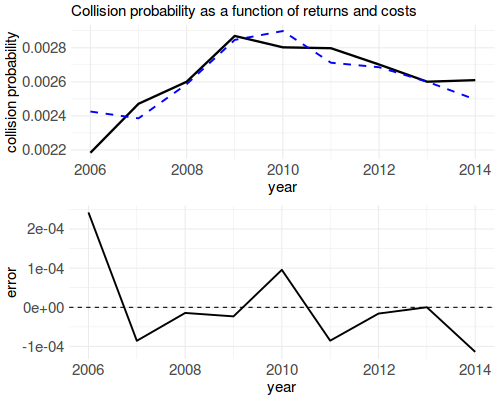
\includegraphics[width=0.7\textwidth]{../../images/risk_return_plot.png}
%	\captionsetup{format=hang}
%	\caption[Open access equilibrium condition model fit]{\textit{Calibration fit.} \\
%		The upper panel shows fitted values (blue dashed line) against actual values (black solid line). The lower panel shows the residuals.
%	}
%	\label{econCalibration}
%\end{figure}
\begin{table}[H]
	\centering
	\begin{tabular}{|l|l|l|l|}
		\hline
		\textit{Economic calibration parameters:}      & \textbf{$a_{L 1}$} & \textbf{$a_{L 2}$} & \textbf{$a_{L 3}$} \\ \hline
		\textit{Parameter values:} & 0.004               & 0.009               & -0.0004 \\ \hline
		\textit{Standard errors:} & 0.002 & 0.002 & 0.001 \\ \hline
	\end{tabular}
	\caption[Parameter values from estimating equation \ref{empiricalEqn}]{Parameter values from estimating equation \ref{empiricalEqn}. All values are rounded to the first non-zero digit.}
	\label{econParms}
\end{table}

If our data perfectly measured the costs and returns of satellite ownership, and our theoretical model held exactly, we would expect $a_{L 1}=1$, $a_{L 2} = 1$, and $a_{L 3} < -1$. Our estimates therefore suggest that our returns and cost series are measured with error or that our theoretical model is missing some important factors, such as constraints on the number of launches possible each period. In this situation, using the raw economic data with the theoretical model could yield overly-pessimistic predictions. To account for this, we adjust our satellite launch cost data to be consistent with the simple open access model by using the estimated parameter values from the economic calibration. Extended Data Table 3 compares the adjusted data to the original series. The adjusted cost data are of the same magnitude as the unadjusted data, but typically smaller. This suggests that the unmodeled factors include cost efficiencies in satellite production, launch, and management, or constraints on launch services available each period, which are consistent with the analytical features we abstract from in our theoretical model. \\

The open access model described so far assumes that any firm which wants to launch a satellite can do so. If launches are limited, as they are in practice, this assumption will be violated. The limits will prevent open access launching from equating the excess return on a satellite with the risk of its destruction. In this way, firms which are able to launch earn rents from having a satellite while the collision risk is below the excess return. The wedge between the collision risk and excess return will reflect the value of those rents. To get a sense of how a binding launch constraint would affect our estimates, we adapt the flow-controlled equilibrium condition from \cite{rao2019diss} to our situation with time-varying parameters.

\begin{equation}
\label{OAfloweqmcond}
L(S_{t+1},D_{t+1}) = \left(1 - \frac{p_t}{F_{t+1} + p_{t+1}} \right) + \frac{\pi_{t+1}}{F_{t+1} + p_{t+1}} - (1+r_t)\frac{F_t}{F_{t+1} + p_{t+1}},
\end{equation}

$p_t$ can be interpreted in two ways. It can be viewed as the implied rent received by a firm which already owns a satellite in $t$ due to launches in $t$ being restricted. It can also be viewed as the implied launch fee paid by a firm which is allotted a launch slot in $t$. In either view, a binding launch constraint results in positive values of $p_t$ and $p_{t+1}$, biasing the coefficients from regression \ref{OAeqm_ch3_2}. $a_{L1}$ is biased toward negative infinity, while $a_{L 2}$ and $a_{L 3}$ are biased toward zero. If the data were free of measurement error and an atomistic homogeneous open access model with a constant discount rate $r$ was correct, we would have $a_{L3} = - (1+r)$. We set the discount rate to be 5\% ($r=0.05$, implying a discount factor of $\beta = (1+r)^{-1} \approx 0.95$). \\

Regardless of the factors missing from the theoretical model, we use equation \ref{empiricalEqn} to recursively calculate the sequence of launch costs implied by the combination of open access, observed launch rates, and observed satellite returns as
\begin{align}
L(S_t,D_t) &= a_{L 1} + a_{L 2} r_{st} + a_{L 3} \frac{F_{t-1}}{F_t} + \epsilon_{r t} \nonumber \\
\implies \hat{F}_t &=	\frac{a_2 \pi_t + a_3 F_{t-1}}{L_t - a_1}.
\label{recursive_impliedcosts}
\end{align}

This ``adjusted cost'' accounts for these missing factors for the historical period. When it exceeds the observed costs, it is likely that the missing factors tend to reflect unobserved costs to launching satellites, such as limited launch availability. When it is below the observed costs, it is likely that the missing factors tend to reflect unobserved returns to launching satellites, such as returns to scale.  \\

Extended Data table 3 shows the observed satellite returns ($\pi_t$), observed launch costs ($F_t$), and implied launch costs ($\hat{F}_t$). The adjusted costs can be interpreted as the costs such that observed launch patterns result from open access under a non-binding launch constraint and with no other unmeasured factors impacting launch costs. Using the adjusted costs instead of the observed costs in the historical sample ensures that our parameter estimates are consistent with our model of open access.\footnote{Estimating the economic parameters using an open access model with a binding launch constraint is challenging as equation \ref{OAeqm_ch3} becomes an inequality, giving sets of open access-consistent parameters rather than a unique combination.}

%\begin{table}[H]
%	\centering
%	\begin{tabular}{@{\extracolsep{5pt}}|l|l|l|l|}
%		\hline 
%		\textit{Year} & \multicolumn{1}{l|}{Observed return} & \multicolumn{1}{l|}{Observed cost} & \multicolumn{1}{l|}{Implied cost} \\ \hline
%		\textit{2006} & 70.44                                & 161.02                             & 194.26                            \\ \hline
%		\textit{2007} & 73.87                                & 185.5                              & 178.88                            \\ \hline
%		\textit{2008} & 85.5                                 & 170                                & 154.86                            \\ \hline
%		\textit{2009} & 93.06                                & 137.81                             & 131.47                            \\ \hline
%		\textit{2010} & 101.51                               & 136.16                             & 140.48                            \\ \hline
%		\textit{2011} & 108.84                               & 166.99                             & 149.09                            \\ \hline
%		\textit{2012} & 114.55                               & 186.88                             & 165.69                            \\ \hline
%		\textit{2013} & 120.25                               & 215.9                              & 170.79                            \\ \hline
%		\textit{2014} & 123.18                               & 254.39                             & 170.68                            \\ \hline
%	\end{tabular}
%	\caption[Launch costs implied by open access model and observed revenues and costs]{Launch costs implied by open access and observed revenues and costs. All values are given in billions of nominal US dollars per year. 2015 is omitted due to the recursive nature of equation \ref{recursive_impliedcosts}. }
%	\label{launchCosts}
%\end{table}


\subsubsection{Algorithms for open access and optimal policy functions}

We generate two sequences of policy functions: one function for each period under consideration, and one sequence for each management regime type. We compute each sequence through backwards induction: beginning at the final period in our projection horizon, and iteratively working backwards to the initial period. This procedure implies ``perfect foresight'' planning under each management regime, i.e. that all agents under any management regime are able to perfectly forecast the sequence of returns, costs, interest rates, launch rates, and other model objects. The perfect foresight assumption is clearly unrealistic, but our purpose is not to show how uncertainty in economic parameters propagates over time. Rather, our purpose is to show how an optimal OUF would vary over time and the time paths of orbital aggregate stocks under different management regimes. Such assumptions are used in integrated assessment models of climate change with similar rationales, e.g. the models studied in \citet{kellykolstad1999, nordhaus2013, IAMsummary}. Our work here is conceptually similar to integrated assessment modeling. \\

To compute the open access time path, we first generate a grid of satellite and debris levels, $(grid_S,grid_D)$. We generate this grid as an expanded Chebyshev grid to reduce numerical errors from interpolation, provide higher fidelity near boundaries, and economize on overall computation time. In contrast to a standard Chebyshev grid, an expanded Chebyshev grid allows for computation (rather than extrapolation) at the boundary points. The formula for the $k^{th}$ expanded Chebyshev node on an interval $[a,b]$ with $n$ points is
\[ x_k = \frac{1}{2}(a+b) + \frac{1}{2}(b-a)\sec\left( \frac{\pi}{2n} \right) \cos\left( \frac{k}{n} - \frac{1}{2n} \right) \]

We set different values of $a$ and $b$ for $S$ and $D$, creating a rectangular grid. The main issue in setting $b$ is ensuring that the time paths we solve for (described in section \ref{genTimePaths}) do not run into or beyond the boundary. To avoid this issue while minimizing the number of points in regions the time paths never reach, we set different $a$ and $b$ bounds for open access and the optimal plan, with the open access grid being strictly larger in both dimensions than the optimal plan grid. \\ 

In general, computing decentralized solutions under open access is simpler than computing the planner's solutions. This is because open access simplifies the continuation value to the cost of launching a satellite. We use \texttt{R} for all simulations, parallelizing where possible. To facilitate convergence of policy and value functions, we normalize the returns and costs parameters so that $\pi_1 = 1$ during computation, and rescale the parameters after the time paths have been generated. \\

We compute optimal value functions by value function iteration on a grid of the state variables $S$ and $D$. We initialize the algorithm with a guess of the value and policy functions. Then, at each point on the grid, we solve the first-order condition for the planner's problem (equation \ref{plannersFOC}). Since there may be multiple solutions, only one of which leads to a global maximum, we then evaluate the value function at each solution (including zero) and select the launch rate attached to the largest level of the value function. Algorithm \ref{vfpfi_algo} describes how we compute the optimal policy and value functions for a given grid and given value function guess $guess(S,D)$, while algorithm \ref{oa_sd_algo} describes how we compute the open access policy and value functions. \\

We construct our initial guess of the planner's value function as the terminal value of the fleet. In the penultimate period, we assume it is not optimal to launch any satellites ($X^*_{T-1} = 0$), making the final fleet size 

\[ S_T = S_{T-1}(1-L(S_T,D_T)) .\]

In the final period ($T$), the payoff of the fleet is $\pi S_T$. Our assumption that it is not optimal to launch any satellites in the penultimate period implies that the one-period returns of a satellite do not cover the cost of building and launching ($\beta \pi_T < F_{T-1}$), which we verify to hold in every period of our data. We use the implied series of $F_t$ given the observed $\pi_t$ and launch rate series in solving for open access and optimal policies.

%To construct the implied series of $F_t$ given the observed $\pi_t$ and launch rate series', we solve equation \ref{OAeqm_ch3_2} using the estimated coefficients from equation \ref{empiricalEqn}. We denote the implied launch cost as $\hat{F}_t$ and the implied rate of return on a satellite as $\hat{r}_{st}$.  \\

\begin{algorithm}
	Set 
	\begin{align*} 
	W_0(S,D) &= guess(S,D), \\
	X_0 &\equiv 0
	\end{align*}
	for all $(S,D) \in (grid_S, grid_D)$
	
	Set $i=1$ and $\delta = 100$ \textit{(some large initial value)}.
	
	\While{$\delta > \epsilon $}{
		At each grid point in $(grid_S,grid_D)$, use a numerical rootfinder to obtain 
		\begin{align*}
		X_i &: W_D(S,D) + S L_D(S,D) \hat{F} - \beta [1 - \delta + G_D(S,D) + m SL_D(S,D)] W_D(S',D') = 0,
		\end{align*} where $W_D(S,D)$ is given by equation \ref{W_Dformula}.
		
		Evaluate $W_i(S,D) = \pi S - \hat{F} X_i + \beta W_{i-1}(S',D')$ at $X_i \cup \{ 0\}$, and select whichever value of $X_i \cup \{ 0\}$ maximizes $W_i(S,D)$. $W_{i-1}(S',D')$ is computed by linear interpolation.
		
		$\delta \leftarrow || W_i(S,D) - W_{i-1}(S,D)||_{\infty}$.\algorithmfootnote{We use $||\cdot||_{\infty}$ for the sup norm.}
		
		%$\delta_{policy} \leftarrow || X^*_i - X_{i-1}||_{\infty}$
		
		i $\leftarrow$ i+1	
	}
	\caption{Value function iteration}\label{vfpfi_algo}
\end{algorithm}

\begin{algorithm}
	Use a numerical rootfinder to find the $X_{t-1}^o$ which solves
	\[ L(S_t,D_t) =  a_{L 1} + a_{L 2} \hat{r}_{st} + a_{L 3} \frac{\hat{F}_{t-1}}{\hat{F}_t}, \]
	using the estimated laws of motion for $S_t$ and $D_t$ as functions of $X_{t-1}$, and the estimated function for $L(S_t,D_t)$.
	
	Approximate $W_i^{\infty}(S,D) = \sum_{t=1}^{\infty} \beta^{t-1} (\pi S_t - \hat{F} X_t^o)$ as $W_i^T(S,D) = \sum_{t=1}^{T-1} \beta^{t-1} (\pi S_t - \hat{F} X_t^*)$ by backwards induction, using the estimated laws of motion for $S_{t+1}$ and $D_{t+1}$ and the estimated function for $L(S_t,D_t)$. We use $T=500$.
	
	\caption{Open access launch plan computation}\label{oa_sd_algo}
\end{algorithm}

\subsubsection{Projected time paths}
\label{genTimePaths}
We use algorithms \ref{vfpfi_algo} and \ref{oa_sd_algo} to compute policy and value functions in each period, and run them sequentially from the final period to the first period to generate a series of policy and value functions for each period's set of economic parameters. Algorithm \ref{pfn_vfn_sequence} describes this process.

\begin{algorithm}
	Set economic parameters to final period values.
	
	Run algorithm \ref{vfpfi_algo} (for an optimal path) or \ref{oa_sd_algo} (for an open access path).
	
	\For{t in T-1:1} {
		Set $i=1$ and $\delta = 100$ \textit{(some large initial value)}. Set $X_{0t} = X_T$.
		\While{$\delta > \epsilon$}{
			Using the value function from the previous step as $W(S_{t+1},D_{t+1})$, calculate
			\begin{align*}
			X^*_{it} &: W_{Dt}(S_t,D_t) + S_t L_D(S_t,D_t) \hat{F}_t - \\
			&~~ \beta [1 - \delta + G_D(S_t,D_t) + m S_tL_D(S_t,D_t)] W_{Dt}(S_{t+1},D_{t+1}) = 0, \\
			&~~ \text{ (for an optimal path, where $W_{Dt}(S,D)$ is given by equation \ref{W_Dformula})},
			\end{align*}
			or
			\[ X_{it}^o : L(S_{t+1},D_{t+1}) =  a_{\ell 1} + a_{\ell 2} \hat{r}_{st} + a_{\ell 3} \frac{\hat{F}_{t-1}}{\hat{F}_t} ~~ \text{ (for an open access path)},\]
			using the estimated laws of motion for $S_{t+1}$ and $D_{t+1}$, the estimated function for $L(S_t,D_t)$, linearly interpolating to compute $W_{t+1}(S_{t+1},D_{t+1})$.
			
			$\delta \leftarrow || X_{it} - X_{i-1 t}||_{\infty}$
		}
		
		If calculating an optimal path, set $W_t(S_t,D_t) = \pi_t S - \hat{F}_t X^* + W_t(S^*_{t+1},D^*_{t+1})$. If calculating an open access path, set $W_t(S_t,D_t) = \pi_t S - \hat{F}_t X^o + W_t(S^o_{t+1},D^o_{t+1})$.
	}
	\caption{Generating a perfect-foresight sequence of policy functions}\label{pfn_vfn_sequence}
\end{algorithm}

It is important to note that when obtaining the sequence of policy functions we do not do backwards induction within each economic time period prior to the final period. Instead, we hold the continuation value ($W(S_{t+1},D_{t+1})$) fixed and iterate on the policy functions, using previous iterations' policies as starting points. This ensures that the continuation value incorporates each period's returns and costs only once until the final period, while allowing for any numerical errors in initial policy solves to be corrected. This type of ``policy iteration'' typically takes 1-2 iterations to converge to within 1$e$-3. Backwards induction on the value function in the final period treats that period's costs and returns as steady state values. This is why we change the notation for the fleet value function for algorithm \ref{pfn_vfn_sequence}, indexing by time to indicate that the launch cost and satellite per-period return are changing in each period. \\

Once we have a sequence of policy functions for each period's economic parameters, we generate time paths by picking a starting condition $(S_0,D_0)$, computing the launch rate $X_0$ by thin-plate spline interpolation of the policy function, using the launch rate to compute the next-period state variables, and repeating the process until the terminal period. Extended Data figure 4 shows the simulated open access and optimal paths of launches, satellites, debris, and collision risk over the in-sample period, 2005-2015, as well as projections from 2016-2040. 

\subsubsection{Accounting for launch availability constraints}
\label{launch_constraint}

% describe physical factors, explain how it would affect the open access allocation and the MEC

The maximum number of satellites which can be launched in a year are limited by a variety of factors, including weather, availability of rockets, and availability of launch sites. We estimate this ``launch constraint'' from the observed data for the historical period, and extrapolate it forward for the projection period. To prevent the model from violating the limited availability of launches, we estimate the launch constraint from the observed historical data and then project it forward. In each historical period, we calculate the maximum number of satellites which can be launched as the cumulative maximum of launch attempts (successes+failures). From the historical calculation, we project the launch constraint forward with a linear time trend and an intercept. Table \ref{lc_coefs} shows the estimated coefficients, and Extended Data figure 6 shows the projected launch constraint time path. \\

\begin{table}[H]
	\centering
	\begin{tabular}{|l|l|l|}
		\hline
		\textit{Launch constraint model parameters:} & Intercept & Time trend \\ \hline
		\textit{Parameter values:}                   & 30.13     & 12.5       \\ \hline
		\textit{Standard errors:}                    & 16.43     & 2.65       \\ \hline
	\end{tabular}
	\caption[Parameter values from linear model of launch constraint]{Parameter values from linear model of launch constraint. All values are rounded to two decimal places. We estimate these coefficients using OLS on the historical launch constraint.}
	\label{lc_coefs}
\end{table}

% explain how this gets handled for the historical period. mention the connection between the adjusted coefficients and the shadow price of launches. adjusted coefficients include the shadow price of launches as well as the effects of ownership shares which are correlated with either satellite returns and costs, or with the shadow price of the launch constraint. By adjusting the historical data to be consistent with this, we ensure that our projections are consistent with open access launching and the observed number of launches while being agnostic to the nature of market frictions during that period. 

In the historical period, we use the adjusted launch costs (described in section \ref{economicCalibrationSection}) When the zero-profit or optimal number of launches exceeds the launch constraint in the projection period, we impose the constraint. If the constraint binds for both the planner and open access firms, then the estimated optimal OUF will be zero. If the constraint binds on open access firms but not on the planner, the optimal OUF will be lower than if the constraint had not bound open access firms.  If we impose the constraint when in reality it would not bind, we will underestimate the optimal OUF. \\


\subsection{Sensitivity analyses of physical equation calibration}
\label{physicsSensitivity}

To study the sensitivity of our conclusions to uncertainty in our physical parameter estimates, we conduct a sensitivity analysis of the model simulations given different physical parameter values. We use a residual bootstrap procedure to obtain sets of alternative parameter values. \\

First, we estimate equations \ref{riskEstimation} and \ref{debLoMEstimation} as described above. Then, we sample from the distribution of residuals to generate ``bootstrap worlds''. We add these residuals to the estimated models to generate bootstrap world outcome variables. Finally, we re-estimate the model using the bootstrap world outcomes to generate alternate sets of physical parameter estimates, and simulate the model under a random sample of those estimates. Algorithm \ref{bootstrap_algo} describes our procedure precisely.\\
\begin{algorithm}
	Estimate equations \ref{riskEstimation} and \ref{debLoMEstimation} to obtain base parameter estimates, $\Phi$, and residuals, $\{(\epsilon_{Lt},\epsilon_{Dt})\}_t$.
	
	Draw from $\{(\epsilon_{Lt},\epsilon_{Dt})\}_t$ with replacement to generate $b=1,\dots,B$ bootstrap resamples $\{(\epsilon_{Lt},\epsilon_{Dt})^b\}_t$.
	
	Generate $B$ bootstrap time series, $L^b(S_t,D_t)$ and $D_{t+1}^b$, using equations \ref{riskEstimation} and \ref{debLoMEstimation} with base estimates $\Phi$ and resampled residuals $\{ (\epsilon_{Lt},\epsilon_{Dt})^b \}_t$.
	
	Re-estimate equations \ref{riskEstimation} and \ref{debLoMEstimation} using $L^b(S_t,D_t)$ and $D_{t+1}^b$ as dependent variables to obtain bootstrap parameter estimates $\{\Phi^b\}_1^B$.
	\caption{Bootstrap procedure}\label{bootstrap_algo}
\end{algorithm}

One issue to note is that, because we estimate equation \ref{riskEstimation} with a constrained procedure and the coefficients are near one of the constraint boundaries, the asymptotic properties of this procedure are difficult to obtain \cite{ketz2018}. Since our goal is not asymptotic analysis of standard errors but rather to generate alternate parameter sets in a principled way for counterfactual simulations, we select the main model estimates as the mean of the bootstrap world parameters. This ensures that our sensitivity analysis selects parameters around the main model estimates. Ultimately this is inconsequential for the outcomes of interest --- collision risk under open access and optimal management, and the resulting OUF --- since the outcomes are endogenous variables which satisfy economic conditions irrespective of the specific physical parameter values. The physical parameter values affect the specific paths of launches, satellites, and debris, but only such that the collision risk continues to satisfy the economic conditions.

\subsection{Projecting the optimal OUF path}

With the calibrated parameter values, we turn to projecting the optimal OUF path. We split this process into two stages. In the first stage, we compute the time paths of the satellite stock, debris stock, and launch rate, given the open access and fleet planner models of orbit use. These describe the projected evolution of the orbital aggregates. In the second stage, we use the computed time paths with the estimated collision probability function and launch cost path to calculate the optimal OUF. The OUF is derived from the same open access and fleet planner models. It describes the amount which a satellite owner would have to be charged every year, beginning from the projection horizon's initial conditions, in order to align their incentives with the fleet planner's.\footnote{This can also be thought of as ``How much of the profits from orbit use currently reflect resource rents which should not have been dissipated?'' } We show the in-sample fit of our open access projections to establish that our approach can approximate the observed history, and then use predictions of space economy revenues and costs from \citep{MSreport} to project out the open access and optimal launch rates given those predictions. \\

We calculate the time path of an optimal OUF from equation \ref{optTax}:

\begin{equation}
\label{optTax}
\tau_t = (L(S^o_{t+1},D^o_{t+1}) - L(S^*_{t+1},D^*_{t+1}))F_{t+1},
\end{equation}

where $S^o_{t+1}$ and $D^o_{t+1}$ are satellite and debris stocks in $t+1$ under open access management, and $S^*_{t+1}$ and $D^*_{t+1}$ are satellite and debris stocks in $t+1$ under optimal management. The optimal OUF is positive whenever the planner would maintain a lower collision probability than firms under open access would. The planner, in turn, will maintain a lower collision probability if the lifetime returns from another satellite in orbit are less than that satellite's expected future damages to other satellites in the fleet. By charging open access firms the marginal external cost of their satellite as an OUF, their incentives are aligned with those of the planner despite the institutional differences. With their incentives aligned, their decisions to launch or not are shifted to optimize the total intertemporal economic value from orbit use rather than their own individual profit. \\

Formally, equation \ref{optTax} can be derived by comparing the open access equilibrium condition (equation \ref{OAeqm_ch3_2}) to the fleet planner's optimality condition for launching (the first-order condition of system of equations \ref{plannersProblem}). These conditions can be written to express the expected loss in satellite value (collision probability multiplied by replacement cost) in terms of economic and, in the case of the optimality condition, physical parameters. Those economic parameters include terms for the current excess return on a satellite in addition to the capital gain or loss from changes in the cost of a replacement satellite. By subtracting the optimal expected loss from the open access expected loss, we recover the additional physical and economic term the social planner accounts for --- the marginal external cost of a satellite. The marginal external cost is the optimal OUF value to levy on each satellite. \\

\subsection{Projecting the effects of active debris removal under open access}

% Brief description of the thought experiments
Finally, we consider the effects of active debris removal technologies on the NPV losses due to open access, shown in Extended Data figure 5. We assume that debris removal is available for zero cost, and that 50\% of all debris is removed from orbit each period once the technology is available. For example, in a scenario where removal begins in 2030, we assume that 50\% of all debris in orbit is removed every year beginning in 2030. We assume debris is removed before it collides with any other orbiting object, and that implementing the removal technology does not require any additional satellites. \\

These assumptions help us bound a ``best case'' removal scenario. In reality, removal will cost more than \$0 per unit removed, will require some additional satellites on orbit to implement, and will not be guaranteed to be successful in all cases. Since debris removal in LEO is not commercially available yet, we experiment with different removal start years between 2021--2034.\\

% Show the changes to laws of motion, open access condition, and planner's condition
The laws of motion with debris removal are
\begin{align}
\label{satelliteLoM_rem}
S_{t+1} &= S_t(1 - L(S_t,D_t(1-R_t)))\mu + X_t \\
\label{debrisLoM_rem}
D_{t+1} &= D_t(1-R_t)(1-\delta) + G(S_t,D_t(1-R_t)) + \gamma A_t + mX_t,
\end{align}

where $R_t = 0.5$ if removal technologies are available and $0$ otherwise.  \\

The open access equilibrium condition is unchanged from the condition without (equation \ref{OAeqm_ch3_2}). The planner's optimality condition with freely-provided debris removal is similar to the condition without (equation \ref{plannersFOC}), but with $(1-R_t)$ terms scaling the debris variable and all derivatives with respect to debris:
\begin{align}
\hspace{-1.25cm}	W_{D,t}(S_t,D_t(1-R_t)) =& - S_t L_D(S_t,D_t(1-R_t))(1-R_t) F_t + \nonumber \\
& \beta [1 - \delta + G_D(S_t,D_t(1-R_t))(1-R_t) + \nonumber \\
& m S_tL_D(S_t,D_t(1-R_t))(1-R_t)] W_{D,t+1}(S_{t+1},D_{t+1}(1-R_{t+1})),
\end{align}
where
\begin{align}
\hspace{-1.75cm}	W_{D,t}(S_t,D_t(1-R_t)) =& \bigg[ \frac{F_{t-1}}{\beta} - \pi_t - (1 - L(S_t,D_t(1-R_t)) - S_t L_S(S_t,D_t(1-R_t)))F_t - \nonumber \\
& \left( \frac{G_S(S_t,D_t(1-R_t)) - m(1 - L(S_t,D_t(1-R_t)) - S_tL_S(S_t,D_t(1-R_t)))}{1 - \delta + G_D(S_t,D_t(1-R_t))(1-R_t) + m L_D(S_t,D_t(1-R_t))(1-R_t)} \right) \cdot \nonumber \\
& L_D(S_t,D_t(1-R_t))(1-R_t) S_t F_t  \bigg] \cdot \nonumber \\
& \left[ \frac{G_S(S_t,D_t(1-R_t)) - m(1 - L(S_t,D_t(1-R_t)) - S_tL_S(S_t,D_t(1-R_t)))}{1 - \delta + G_D(S_t,D_t(1-R_t))(1-R_t) + m L_D(S_t,D_t(1-R_t))(1-R_t)} + m \right]^{-1}.
\end{align}

\section{Supplementary Equations}

\subsection{Derivation of the optimal launch rate}

In this section we derive the equations characterizing the planner's launch rule, equations \ref{plannersFOC} and \ref{W_Dformula}. Period $t$ values are shown with no subscript, and period $t+1$ values are marked with a $'$, e.g. $S_t \equiv S, S_{t+1} \equiv S'$. %For notational simplicity, we keep the economic parameters are constant over time. 
The fleet planner's problem is
\begin{align}
W(S,D) =& \max_{X \geq 0} \{ \pi S - F X + \beta W(S',D') \} \\
\text{s.t. } & ~ S' = S(1-L(S,D)) + X \\
& ~ D' = D (1-\delta) + G(S,D) + \gamma A + m X .
\end{align}

The fleet planner's launch plan will satisfy
\begin{equation}
\label{FOC}
X^* : \beta [ W_S(S',D') + m W_D(S',D') ] = F ,
\end{equation}

that is, the planner will launch until the marginal value to the fleet of a new satellite plus the marginal value to the fleet of its launch debris is equal to the launch cost. \\

Assuming an optimal policy function $X^* = H(S,D)$ exists and applying the envelope condition, we have the following expressions for the fleet's marginal value of another satellite and another piece of debris:
\begin{align}
\label{BS_S}
W_S(S,D) &= \pi + \beta [ W_S(S',D')(1-L(S,D) - SL_S(S,D)) + W_D(S',D')G_S(S,D)] \\
\label{BS_D}
W_D(S,D) &= \beta [ W_D(S',D')(1 - \delta + G_D(S,D)) + W_S(S',D') (-S L_D(S,D)) ]
\end{align}

Rewriting equation \ref{FOC}, we have
\begin{equation}
\label{FOC2}
W_S(S',D') = \left [ \frac{F}{\beta} - m W_D(S',D') \right ]
\end{equation}

Plugging equation \ref{FOC2} into equations \ref{BS_S} and \ref{BS_D},
\begin{align}
\label{BS_S2}
W_S(S,D) &= \pi + F(1 - L(S,D) - SL_S(S,D)) - \beta W_D(S',D') [m(1-L(S,D)-SL_S(S,D)) - G_S(S,D)] \\
\label{BS_D2}
W_D(S,D) &= (-SL_D(S,D)) F + \beta W_D(S',D')[1 - \delta + G_D(S,D) - m(-SL_D(S,D))]
\end{align}

Define the following quantities:
\begin{align*}
\alpha_1(S,D) &= \pi + ( 1 - L(S,D) - SL_S(S,D)) F \\
\alpha_2(S,D) &= -SL_D(S,D)F \\
\Gamma_1(S,D) &= G_S(S,D) -  m ( 1 - L(S,D) - SL_S(S,D))  \\
\Gamma_2(S,D) &= 1 - \delta + G_D(S,D) + mSL_D(S,D). \\
\end{align*}

These allow us to rewrite equations \ref{BS_S2} and \ref{BS_D2} as
\begin{align}
\label{BS_S3}
W_S(S,D) &= \alpha_1(S,D) + \beta \Gamma_1(S,D)W_D(S',D') \\
\label{BS_D3}
W_D(S,D) &= \alpha_2(S,D) + \beta \Gamma_2(S,D) W_D(S',D').
\end{align}

As long as $\delta < 1$, $\Gamma_2(S,D) \neq 0 ~\forall (S,D)$, allowing us to rewrite equation \ref{BS_D3} as
\begin{equation}
\label{BS_D3a}
W_D(S',D') = \frac{W_D(S,D) - \alpha_2(S,D)}{\beta \Gamma_2(S,D)}.
\end{equation}

Plugging equation \ref{BS_D3a} into equation \ref{BS_S3}, we get
\begin{align}
W_S(S,D) &= \alpha_1(S,D) + \beta \Gamma_1(S,D) \frac{W_D(S,D) - \alpha_2(S,D)}{\beta \Gamma_2(S,D)} \nonumber \\
&= \alpha_1(S,D) + \frac{\Gamma_1(S,D)}{\Gamma_2(S,D)} (W_D(S,D) - \alpha_2(S,D)) \nonumber \\
\label{BS_S3a}
\implies W_S(S,D) &= \alpha_1(S,D) - \frac{\Gamma_1(S,D)}{\Gamma_2(S,D)}\alpha_2(S,D) + \frac{\Gamma_1(S,D)}{\Gamma_2(S,D)} W_D(S,D) 
\end{align}

Iterating equation \ref{FOC2} one period backwards and plugging it into equation \ref{BS_S3}, we get
\begin{align}
\frac{'F}{\beta} - m W_D(S,D) &= \alpha_1(S,D) - \frac{\Gamma_1(S,D)}{\Gamma_2(S,D)}\alpha_2(S,D) + \frac{\Gamma_1(S,D)}{\Gamma_2(S,D)} W_D(S,D) \nonumber \\
\label{BS_D4}
\implies W_D(S,D) &= \left[ \frac{'F}{\beta} -  \alpha_1(S,D) - \frac{\Gamma_1(S,D)}{\Gamma_2(S,D)}\alpha_2(S,D) \right] \left[ \frac{\Gamma_1(S,D)}{\Gamma_2(S,D)} + m \right]^{-1}.
\end{align}

Substituting in the forms for $\alpha_1(S,D), \alpha_2(S,D), \Gamma_1(S,D),$ and $\Gamma_2(S,D)$, equation \ref{BS_D3} yields equation \ref{plannersFOC} and equation \ref{BS_D4} yields
\begin{align}
\label{W_Dformula}
W_D(S,D) =& \left[ \frac{'F}{\beta} - \pi - (1 - L(S,D) - S L_S(S,D))F - \frac{G_S(S,D) - m(1 - L(S,D) - SL_S(S,D))}{1 - \delta + G_D(S,D) + m L_D(S,D)}L_D(S,D) S F  \right] \cdot \nonumber \\
& ~~ \left[ \frac{G_S(S,D) - m(1 - L(S,D) - SL_S(S,D))}{1 - \delta + G_D(S,D) + m L_D(S,D)} + m \right]^{-1}.
\end{align}

Combining equation \ref{W_Dformula} with equation \ref{BS_D4} iterated one period forwards, we obtain
\begin{equation*}
L(S',D') = 1 + r_{s}' - (1+r)\frac{F}{F'} - \xi(S',D'),
\end{equation*}
where
\begin{align*}
&\xi(S',D')  = S'L_S(S',D')F' + \frac{\pi - rF - L(S,D)F - S L_S(S,D) F}{\beta (1- \delta + G_D(S',D') + mL_D(S',D')S' )} \\ 
& ~~~~~ -\frac{\beta G_S(S',D') + m(1 - L(S',D') - S'L_S(S',D'))}{\beta (1- \delta + G_D(S',D') + mL_D(S',D')S' )}L_D(S',D')S'F'.
%&\xi(S_{t+1},D_{t+1})  = S_{t+1}L_S(S_{t+1},D_{t+1})F_{t+1} + \frac{\pi_t - rF_t - L(S_t,D_t)F_t - S_t L_S(S_t,D_t) F_t}{\beta (1- \delta + G_D(S_{t+1},D_{t+1}) + mL_D(S_{t+1},D_{t+1})S_{t+1} )} \\ 
%& ~~~~~ -\frac{\beta G_S(S_{t+1},D_{t+1}) + m(1 - L(S_{t+1},D_{t+1}) - S_{t+1}L_S(S_{t+1},D_{t+1}))}{\beta (1- \delta + G_D(S_{t+1},D_{t+1}) + mL_D(S_{t+1},D_{t+1})S_{t+1} )}L_D(S_{t+1},D_{t+1})S_{t+1}F_{t+1}.
\end{align*}

\section{Supplementary Discussion}

\subsection{Interpreting the optimal OUF and long-run industry value paths}

Figure 2 in the main text shows the NPV gains from beginning optimal management in different years, and the permanent orbit use value losses in 2040 from delaying optimal management. The permanent orbit use value is the discounted value of the satellite fleet over the long-run, accounting for losses and replacements. \\

The discontinuous jumps in NPV in figure 2 reflect the immediate effect of reducing launch activity while the satellite and debris stocks are suboptimally high. The change in launch activity increases the NPV by reducing the cost outflows each year. Since open access launching results in excess satellites and debris, the benefits of optimal management continue to accrue gradually as the satellite and debris stocks draw down. Extended Data figure 4 shows these launch rate dynamics for a 2006 optimal management start. \\

The fact that the optimal OUF, shown in Extended Data figure 10, rises over time is an indication of the restored value of orbit use due to optimal management (orbital rents). Intuitively, firms fully dissipate orbital rents in an open access equilibrium, as those rents act as an incentive to enter. To counter the growth in the incentive to enter due to restored orbital rents, the OUF must also rise over time. A firm which enters the commons early on (say, 2020) will pay a lower initial fee than a firm which enters later on (say, 2030) because the early entrant is paying to use a more congested environment. \\

Though our modeling procedure abstracts from many economic and physical complications, our optimal OUF and long-run industry value estimates are likely robust to these limitations and on the correct order of magnitude with the correct qualitative features. On the OUF side, given that the projected optimal launch path beginning from the projected 2020 state of LEO involves cessation of launch activity, the estimated OUF in 2020 needs only to be large enough to deter launches, particularly those likely to generate large and suboptimal increases in collision risk.  While satellite operators in LEO are heterogeneous and represent diverse interests, we estimate an optimal averaged-across-LEO-use-cases per-satellite per-year fee beginning at approximately \$13,500 USD and growing over time. \cite{letiziaetal2017} identify that the majority of collision risk increases in the near future will be driven by satellite constellation operators. For an entity planning to launch a constellation of 600 satellites, our OUF amounts to an additional yearly expenditure beginning at \$8.1 million USD --- likely enough to prompt serious reconsideration of the size and nature of the constellation. On the industry value side, the global satellite sector currently produces approximately \$0.15 trillion USD in revenues, and is anticipated to grow to \$2 trillion USD in revenues and costs by 2040 \citep{MSreport}. A decrease in collision risk which leads to a 10\% increase in the per-year economic value of the satellite sector would immediately add 10\% to the sector's NPV. Our model projects that collision risk in 2040 will decrease by roughly 33\% (compared to BAU) under an optimal management plan beginning in 2020. This reduction collision risk would cut collision-related replacement costs, increase the expected lifespan of satellites in orbit, and reduce collision-related disruptions in the stream of satellite-related economic returns. Given this, long-run industry value in 2040 on the order of single-digit trillions of USD seems plausible.

% TALK THROUGH THE FIGURES
%While the historical fit of the open access model is not exact, it is on the right order of magnitude and exhibits the correct trends. Our model is highly simplified and aggregated, and does not include a detailed model of orbital mechanics (necessary to correctly propagate the state variables over time) or a detailed model of launch industry dynamics (necessary to correctly model the idiosyncrasies of the launch path).\footnote{For example, on the physical side we abstract from different types of objects in orbit and time variation in their inclinations and relative velocities. On the economic side, we abstract from market power in the launch industry, the different types of commercial industries using satellites, and increasing returns to scale in satellite launch and ownership.} Our focus is on obtaining approximations which are the correct order of magnitude and exhibit the correct time trends. Future research which integrates detailed physical models of orbital mechanics with detailed models of satellite and launch industry dynamics will be required to provide precise values for OUFs and NPV loss.

\subsection{Open access and active debris removal}

The introduction of debris removal makes both open access firms and the planner launch additional satellites. However, the planner launches considerably fewer additional satellites than open access firms. The immediate decrease in debris when removal becomes available induces new launches until the collision risk is once again equated with the excess return on a satellite. Extended Data figure 5a--d shows the effects of debris removal beginning in 2029 on satellite and debris accumulation under open access and a range of optimal management paths. The removal-induced additional launching leads to a higher steady-state satellite stock and a lower steady-state debris stock under open access and optimal management. The amount of debris removed in our ``50\% removal'' scenario is substantially larger under open access than the optimal plan as there is more debris in orbit under open access. \\

Though debris removal allows open access to sustain more satellites in orbit, over time collision risk returns to the equilibrium level. The costs of additional launches erodes some of the NPV gains due to reduced risk. Extended Data figure 5e shows the percentage change in open-access NPV loss due to the introduction of debris removal in 2029, as a fraction of the potential gain from implementing the optimal plan in 2020. Extended Data figure 5f summarizes the minimum, mean, and maximum changes in long-run industry value losses due to open access with removal beginning in each year in 2021--2034. On average, debris removal beginning in the 2021--2034 window reduces open access NPV losses by about 1.65\% relative to a counterfactual world without removal. When optimal management begins ahead of debris removal, the NPV losses tend to be reduced (negative changes). When optimal management begins after debris removal, the NPV losses tend to be increased (positive changes). The increase in NPV losses in the latter scenario is driven by the costs of additional launching under open access, both immediately following the initial debris reduction and to sustain the larger satellite population. Due to open access, firms will take advantage of lower collision risk due to debris removal by launching satellites until there are no more profits from launching new satellites. When the planner is in charge of launching before debris removal begins, they do not waste resources by launching to dissipate the gains from debris removal.

\subsection{Unmodeled physical and economic factors}
\label{disc_unmodeledeconphys}
%Paragraph 3: high-level overview of limitations. Launch constraint, which we linearly project out and allow the economic parameter estimation to incorporate shadow values for; future constellations are mini-planners, biasing our estimates; placement of satellites: environmentally conservative (assuming current patterns continue overstates level of risk for both planner and open access), economically generous (assuming current patterns continue underestimates difference between planner and open access) -- our OUF calculation can be understood as a lower bound on continuing to have satellites placed less-optimally than a planner would.
In addition to the limitations imposed by modeling spatially and temporally heterogeneous physical and economic processes at an aggregated level, there are three main analytical limitations pertaining to unobservables in the past and present and unknowables in the future: launch market frictions, constellations (coordinated systems of satellites intended to serve a common purpose), and satellite placement. These limitations may make our OUF estimates lower bounds on the true values required to induce optimal orbit use, as we describe below.\\ 

Our conclusions about the suboptimality of open access to orbit and the necessity of a globally-coordinated OUF (or policies equivalent to one) are robust to these limitations.  The fundamental problem creating the need for policies equivalent to a globally-coordinated OUF is the lack of legally-enforceable property rights over orbits.\footnote{The geostationary belt is the exception to this statement. In general, however, there is no globally-coordinated procedure for allocating orbital paths, or even a globally-agreed-upon definition of an orbital path property right.} The lack of property rights prevents satellite owners from internalizing the costs they impose on others through collision risk and debris creation. The same issue manifests in other common-resource settings, such as fisheries \cite{gordon1954}. \\

Our economic model is founded on the assumption that all agents who want to launch satellites are able to do so with no frictions. In practice, there are factors other than orbital property rights and willingness-to-pay which limit agents' access to orbit, such as limited availability of launch windows and rockets. These factors constrain humanity's ability to launch satellites. To ensure that our simulations do not violate this launch constraint in observed years, we calculate the launch constraint in each observed period as the cumulative maximum number of launches observed so far. The shadow value of the launch constraint is recovered in the economic parameter calibration process, but the individual factors are not identifiable from the data. We then fit a linear time trend to the observed launch constraint, and project it into the future. To the extent that the launch constraint will be relaxed faster than a linear trend would predict, our estimates are economically conservative, i.e. we assume fewer launches than may occur, which biases our estimated OUF downward. \\

Our economic model is also founded on the simplifying assumption of ``one satellite per firm''. In practice, there are a number of firms which own constellations or fleets of satellites. However, unless a single firm owned all satellites in orbit, orbit users would not internalize the full scope of the externality they impose on others. To the extent that the observed data reflects agents internalizing those externalities due to ownership of multiple satellites, our economic parameter estimates would entangle those factors with the estimated launch constraint shadow value. Our projections of single-satellite-owning firms' responses to increases in satellite profitability would therefore be attenuated toward zero, making our projections environmentally conservative, i.e. closer to an environmental ``worst-case'' analysis. However, the same assumption also increases the optimal OUF we estimate. \\

Lastly, our model abstracts entirely away from the question of satellite placement. That is, two orbital objects within a given volume shell can be placed in orbits such that at one extreme they are guaranteed to collide, or at the other extreme they will never collide. Our projections are based on collision rate estimates which are calculated using historical placement patterns. Thus, our projections assume that the systematic factors which resulted in current object placements will continue into the future. While technology and constellation ownership are likely to lead to improvements in placement patterns our collision risk projections would be biased for both the open access and optimal launch paths. However, the magnitude of the gap between open access and optimal collision risk may actually be understated by this issue. To the extent that economic agents have the placement margin available to them it is induces another externality, similar in spirit but different in detail to the orbit use externality we describe in this article, wherein firms do not account for the full magnitude of orbital-use efficiency losses due to their placement. A fleet planner who coordinated all satellites in orbit would account for such placement-related externalities. By taking advantage of any efficiencies in placement, would be able to reduce collision rates below what open access satellite owners would have an incentive to consider. Thus, while the inclusion of a placement margin may reduce levels of collision risk, the differences in collision risk between open access and optimal use may increase, which would make our OUF estimates a lower bound on average.\footnote{While some regimes in a spatially-differentiated orbit model may have lower OUF values than the ones we calculate here, the average OUF value across all regimes will likely be larger.}


\subsection{Consequences of measurement error and misspecification}

\subsubsection{Measurement error in satellite and debris counts}
\label{physicsMeasurementError}

%Random measurement error in the satellite or debris data would bias our estimates of physical parameters toward zero. 
Limitations of sensor technology suggest that the debris counts are lower-bound estimates. To the extent that this biases the collision probability and debris counts downward, it will bias the estimated decay rate, collision probability parameters, fragmentation parameters, and launch debris weakly downwards. Since downward bias in the physical parameters makes collisions and missile tests appear to cause less congestion than they actually do, the open access and optimal launch rates will be inflated.\\

Downward bias in the collision probability data will bias the economic parameter estimates weakly downwards as well. This will to some degree offset the inflation in the launch rate caused by the physical parameter underestimation, though the exact extent of the offset is not clear. \\

In general, measurement error in the collision probability data also causes the nonnegativity constraint on the collision probability parameters ($\alpha_{SS}$ and $\alpha_{SD}$) to bind in some bootstrap replications. This causes issues of the type described in \cite{ketz2018} in obtaining asymptotic standard errors.

\subsubsection{Collision probability model misspecification}

We assume that the collision probability model has constant parameters. Changes in patterns of satellite placement, construction, and ownership structures lead to changes over time in the physical primitives reflected in $\alpha_{SS}$ and $\alpha_{SD}$. The ``net'' convexity or concavity of the time path of the primitives will determine whether the constant approximations over or understate the true time-varying parameters in any period on average. A convex time path --- low values initially and high values later on --- will be overestimated on average, while a concave time path --- high values initially, with slow increases over time --- will be underestimated on average. \\

The misspecification causes two problems with simulation and inference. First, underestimation will inflate launch rate projections and overestimation will deflate them. However, because the deflation affects both open access and optimal launch rates in the same way, the simulated optimal OUF will not be affected. Second, underestimation may cause the nonnegativity constraint on the collision probability parameters to bind in some bootstrap replications, causing the same types of asymptotic issues as measurement error.

\subsubsection{Measurement error in returns and costs}
\label{attenuationFactors}

We take the returns and costs of satellite ownership from the data used in \citet{wienzierl2018}, which aggregate revenues from all commercial satellites in orbit. By including more than just LEO satellites, the direct returns and costs data overstate the returns to LEO paths. The economic parameter estimates therefore reflect a ``LEO share'' coefficient on the revenue data between $0$ and $1$. The LEO share coefficient attenuates the estimates of $a_{L 1}$, $a_{L 2}$, and $a_{L 3}$.


%%% Each figure should be on its own page
\begin{figure}
\centering
\includegraphics[width=\textwidth]{example-image}
\caption{First figure}
\end{figure}

\begin{figure}
\centering

\includegraphics[width=\textwidth]{frog}
\caption{Second figure}
\end{figure}

%\begin{table}\centering
%\caption{This is a table}
%
%\begin{tabular}{lrrr}
%Species & CBS & CV & G3 \\
%\midrule
%1. Acetaldehyde & 0.0 & 0.0 & 0.0 \\
%2. Vinyl alcohol & 9.1 & 9.6 & 13.5 \\
%3. Hydroxyethylidene & 50.8 & 51.2 & 54.0\\
%\bottomrule
%\end{tabular}
%\end{table}

%%% Add this line AFTER all your figures and tables
\FloatBarrier


\dataset{dataset_one.txt}{Type or paste caption here.}

\dataset{dataset_two.txt}{Type or paste caption here. Adding longer text to show what happens, to decide on alignment and/or indentations for multi-line or paragraph captions.}

\bibliography{../../memos/database}

\end{document}